\chapter{Results}
In the end of the previous chapter we introduced the two observables that we explore in our lattice simulation and demonstrated the methods that lead to their continuum extrapolation. We now present the resulting measurements of the mass of the $x$ field and the derivative of the cusp anomaly. We further expose the data for additional simulations performed for $LM=6$ and without a \names{Wilson} term, respectively, to check for finite volume effects and the influence of fermion doublers.
%
%
%
%  - - - - - -     Masses  - - - - - - - -
%
%
%
\section[Mass of the x field]{Mass of the x field}
To estimate the mass of the $x$ field we proceed as presented in section \ref{sec: xx_corr} by calculating the effective masses for the various lattices sizes under consideration. For every fixed $g$ we do a continuum extrapolation (\autoref{fig: mx_Lm4_cont_lim}) and plot $m_{x}^{2}/m^{2}$ over $g$ in \autoref{fig: mx_vs_g_Lm4}. The data points are afflicted with large errorbars. This is because the correlation functions are highly fluctuating and the mass therefore is a challenging observable with a lot of statistical noise that needs a high amount of replica to give good estimates. Nonetheless, we observe for $5<g<100$ $(0.2<g_{\rm c}<4)$\footnote{See section \ref{sec: res_cusp} for the meaning of $g_{\rm c}$.} our data overestimates the mass compared to the perturbative large $g$ prediction ((\ref{eq: m_x}) and dotted line in \autoref{fig: mx_vs_g_Lm4}), but it follows the predicted bending down for smaller couplings. The deviation for the point at $g=5$ $(g_{\rm c}=4)$ could be due to the fact that we do not have as many replica for the various lattice sizes for this particular $g$ value and thus not such a good estimate as for the other values. The same is true for $g=5$ $(g_{\rm c}=0.2)$ where additionally the reweighting might also conflict the mass measurement. The remaining points qualitatively follow the bending down, but are larger than the mass prediction. An explanation could be given by the subtraction of the non-connected part of the correlator in (\ref{eq: conn_corr}) which might be not exact. This is checked by considering simulations without a \names{Wilson} term in section \ref{sec: sys_errors}. There the $SO(2)$ symmetry is unbroken and the correlator coincides with its connected part. 
%
%
%
\begin{figure}
\centering
% This file was created by matlab2tikz.
%
%The latest updates can be retrieved from
%  http://www.mathworks.com/matlabcentral/fileexchange/22022-matlab2tikz-matlab2tikz
%where you can also make suggestions and rate matlab2tikz.
%
\definecolor{mycolor1}{rgb}{0.00000,0.44700,0.74100}%
\definecolor{mycolor2}{rgb}{0.85000,0.32500,0.09800}%
\definecolor{mycolor3}{rgb}{0.92900,0.69400,0.12500}%
\definecolor{mycolor4}{rgb}{0.49400,0.18400,0.55600}%
\definecolor{mycolor5}{rgb}{0.46600,0.67400,0.18800}%
\definecolor{mycolor6}{rgb}{0.63500,0.07800,0.18400}%
\definecolor{mycolor7}{rgb}{0.30100,0.74500,0.93300}%
%
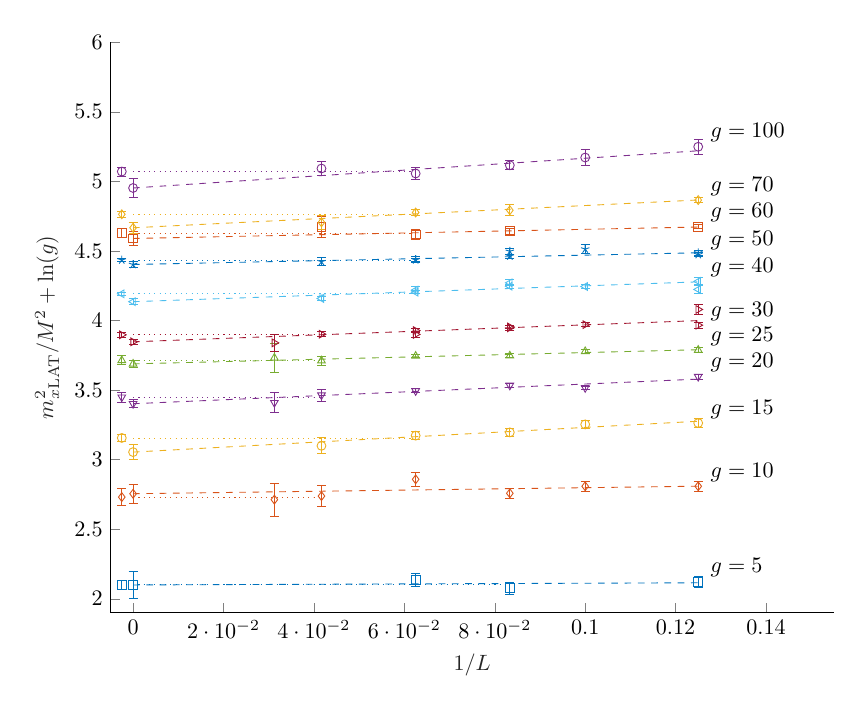
\begin{tikzpicture}[thick,scale=0.8, every node/.style={scale=1}]

\begin{axis}[%
width=4.521in,
height=3.566in,
at={(0.758in,0.481in)},
scale only axis,
xmin=-0.005,
xmax=0.155,
xlabel style={font=\color{white!15!black}},
xlabel={$1/L$},
ymin=1.9,
ymax=6,
ylabel style={font=\color{white!15!black}},
ylabel={$m_{x{\rm LAT}}^2/M^2 + \ln(g)$},
axis background/.style={fill=white},
axis x line*=bottom,
axis y line*=left
]
\addplot [color=mycolor1, dotted, forget plot]
  table[row sep=crcr]{%
0	2.10279104542099\\
0.00125	2.10279104542099\\
0.0025	2.10279104542099\\
0.00375	2.10279104542099\\
0.005	2.10279104542099\\
0.00625	2.10279104542099\\
0.0075	2.10279104542099\\
0.00875	2.10279104542099\\
0.01	2.10279104542099\\
0.01125	2.10279104542099\\
0.0125	2.10279104542099\\
0.01375	2.10279104542099\\
0.015	2.10279104542099\\
0.01625	2.10279104542099\\
0.0175	2.10279104542099\\
0.01875	2.10279104542099\\
0.02	2.10279104542099\\
0.02125	2.10279104542099\\
0.0225	2.10279104542099\\
0.02375	2.10279104542099\\
0.025	2.10279104542099\\
0.02625	2.10279104542099\\
0.0275	2.10279104542099\\
0.02875	2.10279104542099\\
0.03	2.10279104542099\\
0.03125	2.10279104542099\\
0.0325	2.10279104542099\\
0.03375	2.10279104542099\\
0.035	2.10279104542099\\
0.03625	2.10279104542099\\
0.0375	2.10279104542099\\
0.03875	2.10279104542099\\
0.04	2.10279104542099\\
0.04125	2.10279104542099\\
0.0425	2.10279104542099\\
0.04375	2.10279104542099\\
0.045	2.10279104542099\\
0.04625	2.10279104542099\\
0.0475	2.10279104542099\\
0.04875	2.10279104542099\\
0.05	2.10279104542099\\
0.05125	2.10279104542099\\
0.0525	2.10279104542099\\
0.05375	2.10279104542099\\
0.055	2.10279104542099\\
0.05625	2.10279104542099\\
0.0575	2.10279104542099\\
0.05875	2.10279104542099\\
0.06	2.10279104542099\\
0.06125	2.10279104542099\\
0.0625	2.10279104542099\\
0.06375	2.10279104542099\\
0.065	2.10279104542099\\
0.06625	2.10279104542099\\
0.0675	2.10279104542099\\
0.06875	2.10279104542099\\
0.07	2.10279104542099\\
0.07125	2.10279104542099\\
0.0725	2.10279104542099\\
0.07375	2.10279104542099\\
0.075	2.10279104542099\\
0.07625	2.10279104542099\\
0.0775	2.10279104542099\\
0.07875	2.10279104542099\\
0.08	2.10279104542099\\
0.08125	2.10279104542099\\
0.0825	2.10279104542099\\
};
\addplot [color=mycolor1, dashed, forget plot]
  table[row sep=crcr]{%
0	2.09960348442947\\
0.00125	2.09976084054418\\
0.0025	2.09991819665889\\
0.00375	2.1000755527736\\
0.005	2.10023290888831\\
0.00625	2.10039026500303\\
0.0075	2.10054762111774\\
0.00875	2.10070497723245\\
0.01	2.10086233334716\\
0.01125	2.10101968946187\\
0.0125	2.10117704557658\\
0.01375	2.10133440169129\\
0.015	2.101491757806\\
0.01625	2.10164911392072\\
0.0175	2.10180647003543\\
0.01875	2.10196382615014\\
0.02	2.10212118226485\\
0.02125	2.10227853837956\\
0.0225	2.10243589449427\\
0.02375	2.10259325060898\\
0.025	2.10275060672369\\
0.02625	2.10290796283841\\
0.0275	2.10306531895312\\
0.02875	2.10322267506783\\
0.03	2.10338003118254\\
0.03125	2.10353738729725\\
0.0325	2.10369474341196\\
0.03375	2.10385209952667\\
0.035	2.10400945564138\\
0.03625	2.10416681175609\\
0.0375	2.10432416787081\\
0.03875	2.10448152398552\\
0.04	2.10463888010023\\
0.04125	2.10479623621494\\
0.0425	2.10495359232965\\
0.04375	2.10511094844436\\
0.045	2.10526830455907\\
0.04625	2.10542566067378\\
0.0475	2.1055830167885\\
0.04875	2.10574037290321\\
0.05	2.10589772901792\\
0.05125	2.10605508513263\\
0.0525	2.10621244124734\\
0.05375	2.10636979736205\\
0.055	2.10652715347676\\
0.05625	2.10668450959147\\
0.0575	2.10684186570619\\
0.05875	2.1069992218209\\
0.06	2.10715657793561\\
0.06125	2.10731393405032\\
0.0625	2.10747129016503\\
0.06375	2.10762864627974\\
0.065	2.10778600239445\\
0.06625	2.10794335850916\\
0.0675	2.10810071462388\\
0.06875	2.10825807073859\\
0.07	2.1084154268533\\
0.07125	2.10857278296801\\
0.0725	2.10873013908272\\
0.07375	2.10888749519743\\
0.075	2.10904485131214\\
0.07625	2.10920220742685\\
0.0775	2.10935956354156\\
0.07875	2.10951691965628\\
0.08	2.10967427577099\\
0.08125	2.1098316318857\\
0.0825	2.10998898800041\\
0.08375	2.11014634411512\\
0.085	2.11030370022983\\
0.08625	2.11046105634454\\
0.0875	2.11061841245925\\
0.08875	2.11077576857397\\
0.09	2.11093312468868\\
0.09125	2.11109048080339\\
0.0925	2.1112478369181\\
0.09375	2.11140519303281\\
0.095	2.11156254914752\\
0.09625	2.11171990526223\\
0.0975	2.11187726137694\\
0.09875	2.11203461749166\\
0.1	2.11219197360637\\
0.10125	2.11234932972108\\
0.1025	2.11250668583579\\
0.10375	2.1126640419505\\
0.105	2.11282139806521\\
0.10625	2.11297875417992\\
0.1075	2.11313611029463\\
0.10875	2.11329346640935\\
0.11	2.11345082252406\\
0.11125	2.11360817863877\\
0.1125	2.11376553475348\\
0.11375	2.11392289086819\\
0.115	2.1140802469829\\
0.11625	2.11423760309761\\
0.1175	2.11439495921232\\
0.11875	2.11455231532703\\
0.12	2.11470967144175\\
0.12125	2.11486702755646\\
0.1225	2.11502438367117\\
0.12375	2.11518173978588\\
0.125	2.11533909590059\\
};
\addplot [color=mycolor1, draw=none, mark=square, mark options={solid, mycolor1}, forget plot]
 plot [error bars/.cd, y dir = both, y explicit]
 table[row sep=crcr, y error plus index=2, y error minus index=3]{%
0	2.09960348442947	0.0940854482495643	0.0940854482495643\\
-0.0025	2.10279104542099	0.032939252161526	0.032939252161526\\
0.125	2.12368661211111	0.0384201229418747	0.0384201229418747\\
0.0833333333333333	2.07692668955786	0.0442154356693399	0.0442154356693399\\
0.0625	2.13504661264345	0.0493770815069211	0.0493770815069211\\
};
\node[right, align=left]
at (axis cs:0.126,2.224) {$g = 5$};
\addplot [color=mycolor2, dotted, forget plot]
  table[row sep=crcr]{%
0	2.73119370649015\\
0.00125	2.73119370649015\\
0.0025	2.73119370649015\\
0.00375	2.73119370649015\\
0.005	2.73119370649015\\
0.00625	2.73119370649015\\
0.0075	2.73119370649015\\
0.00875	2.73119370649015\\
0.01	2.73119370649015\\
0.01125	2.73119370649015\\
0.0125	2.73119370649015\\
0.01375	2.73119370649015\\
0.015	2.73119370649015\\
0.01625	2.73119370649015\\
0.0175	2.73119370649015\\
0.01875	2.73119370649015\\
0.02	2.73119370649015\\
0.02125	2.73119370649015\\
0.0225	2.73119370649015\\
0.02375	2.73119370649015\\
0.025	2.73119370649015\\
0.02625	2.73119370649015\\
0.0275	2.73119370649015\\
0.02875	2.73119370649015\\
0.03	2.73119370649015\\
0.03125	2.73119370649015\\
0.0325	2.73119370649015\\
0.03375	2.73119370649015\\
0.035	2.73119370649015\\
0.03625	2.73119370649015\\
0.0375	2.73119370649015\\
0.03875	2.73119370649015\\
0.04	2.73119370649015\\
0.04125	2.73119370649015\\
};
\addplot [color=mycolor2, dashed, forget plot]
  table[row sep=crcr]{%
0	2.75527593509874\\
0.00125	2.75581784221291\\
0.0025	2.75635974932708\\
0.00375	2.75690165644125\\
0.005	2.75744356355542\\
0.00625	2.75798547066959\\
0.0075	2.75852737778376\\
0.00875	2.75906928489793\\
0.01	2.75961119201211\\
0.01125	2.76015309912628\\
0.0125	2.76069500624045\\
0.01375	2.76123691335462\\
0.015	2.76177882046879\\
0.01625	2.76232072758296\\
0.0175	2.76286263469713\\
0.01875	2.7634045418113\\
0.02	2.76394644892548\\
0.02125	2.76448835603965\\
0.0225	2.76503026315382\\
0.02375	2.76557217026799\\
0.025	2.76611407738216\\
0.02625	2.76665598449633\\
0.0275	2.7671978916105\\
0.02875	2.76773979872467\\
0.03	2.76828170583884\\
0.03125	2.76882361295302\\
0.0325	2.76936552006719\\
0.03375	2.76990742718136\\
0.035	2.77044933429553\\
0.03625	2.7709912414097\\
0.0375	2.77153314852387\\
0.03875	2.77207505563804\\
0.04	2.77261696275221\\
0.04125	2.77315886986639\\
0.0425	2.77370077698056\\
0.04375	2.77424268409473\\
0.045	2.7747845912089\\
0.04625	2.77532649832307\\
0.0475	2.77586840543724\\
0.04875	2.77641031255141\\
0.05	2.77695221966558\\
0.05125	2.77749412677975\\
0.0525	2.77803603389393\\
0.05375	2.7785779410081\\
0.055	2.77911984812227\\
0.05625	2.77966175523644\\
0.0575	2.78020366235061\\
0.05875	2.78074556946478\\
0.06	2.78128747657895\\
0.06125	2.78182938369312\\
0.0625	2.7823712908073\\
0.06375	2.78291319792147\\
0.065	2.78345510503564\\
0.06625	2.78399701214981\\
0.0675	2.78453891926398\\
0.06875	2.78508082637815\\
0.07	2.78562273349232\\
0.07125	2.78616464060649\\
0.0725	2.78670654772066\\
0.07375	2.78724845483484\\
0.075	2.78779036194901\\
0.07625	2.78833226906318\\
0.0775	2.78887417617735\\
0.07875	2.78941608329152\\
0.08	2.78995799040569\\
0.08125	2.79049989751986\\
0.0825	2.79104180463403\\
0.08375	2.79158371174821\\
0.085	2.79212561886238\\
0.08625	2.79266752597655\\
0.0875	2.79320943309072\\
0.08875	2.79375134020489\\
0.09	2.79429324731906\\
0.09125	2.79483515443323\\
0.0925	2.7953770615474\\
0.09375	2.79591896866157\\
0.095	2.79646087577575\\
0.09625	2.79700278288992\\
0.0975	2.79754469000409\\
0.09875	2.79808659711826\\
0.1	2.79862850423243\\
0.10125	2.7991704113466\\
0.1025	2.79971231846077\\
0.10375	2.80025422557494\\
0.105	2.80079613268912\\
0.10625	2.80133803980329\\
0.1075	2.80187994691746\\
0.10875	2.80242185403163\\
0.11	2.8029637611458\\
0.11125	2.80350566825997\\
0.1125	2.80404757537414\\
0.11375	2.80458948248831\\
0.115	2.80513138960248\\
0.11625	2.80567329671666\\
0.1175	2.80621520383083\\
0.11875	2.806757110945\\
0.12	2.80729901805917\\
0.12125	2.80784092517334\\
0.1225	2.80838283228751\\
0.12375	2.80892473940168\\
0.125	2.80946664651585\\
};
\addplot [color=mycolor2, draw=none, mark=diamond, mark options={solid, mycolor2}, forget plot]
 plot [error bars/.cd, y dir = both, y explicit]
 table[row sep=crcr, y error plus index=2, y error minus index=3]{%
0	2.75527593509874	0.0679665829360463	0.0679665829360463\\
-0.0025	2.73119370649015	0.0626053188900369	0.0626053188900369\\
0.125	2.80909615232382	0.0359980370190172	0.0359980370190172\\
0.1	2.80890117076868	0.0382287436885021	0.0382287436885021\\
0.0833333333333333	2.75829105850798	0.0369545821801482	0.0369545821801482\\
0.0625	2.85863457057082	0.0522555359080003	0.0522555359080003\\
0.0416666666666667	2.73843799740069	0.0740037317295332	0.0740037317295332\\
0.03125	2.7129591799931	0.117409415024243	0.117409415024243\\
};
\node[right, align=left]
at (axis cs:0.126,2.909) {$g = 10$};
\addplot [color=mycolor3, dotted, forget plot]
  table[row sep=crcr]{%
0	3.15612314071118\\
0.00125	3.15612314071118\\
0.0025	3.15612314071118\\
0.00375	3.15612314071118\\
0.005	3.15612314071118\\
0.00625	3.15612314071118\\
0.0075	3.15612314071118\\
0.00875	3.15612314071118\\
0.01	3.15612314071118\\
0.01125	3.15612314071118\\
0.0125	3.15612314071118\\
0.01375	3.15612314071118\\
0.015	3.15612314071118\\
0.01625	3.15612314071118\\
0.0175	3.15612314071118\\
0.01875	3.15612314071118\\
0.02	3.15612314071118\\
0.02125	3.15612314071118\\
0.0225	3.15612314071118\\
0.02375	3.15612314071118\\
0.025	3.15612314071118\\
0.02625	3.15612314071118\\
0.0275	3.15612314071118\\
0.02875	3.15612314071118\\
0.03	3.15612314071118\\
0.03125	3.15612314071118\\
0.0325	3.15612314071118\\
0.03375	3.15612314071118\\
0.035	3.15612314071118\\
0.03625	3.15612314071118\\
0.0375	3.15612314071118\\
0.03875	3.15612314071118\\
0.04	3.15612314071118\\
0.04125	3.15612314071118\\
0.0425	3.15612314071118\\
0.04375	3.15612314071118\\
0.045	3.15612314071118\\
0.04625	3.15612314071118\\
0.0475	3.15612314071118\\
0.04875	3.15612314071118\\
0.05	3.15612314071118\\
0.05125	3.15612314071118\\
0.0525	3.15612314071118\\
0.05375	3.15612314071118\\
0.055	3.15612314071118\\
0.05625	3.15612314071118\\
0.0575	3.15612314071118\\
0.05875	3.15612314071118\\
0.06	3.15612314071118\\
0.06125	3.15612314071118\\
0.0625	3.15612314071118\\
};
\addplot [color=mycolor3, dashed, forget plot]
  table[row sep=crcr]{%
0	3.05440888866837\\
0.00125	3.05662703781743\\
0.0025	3.05884518696648\\
0.00375	3.06106333611553\\
0.005	3.06328148526458\\
0.00625	3.06549963441363\\
0.0075	3.06771778356268\\
0.00875	3.06993593271174\\
0.01	3.07215408186079\\
0.01125	3.07437223100984\\
0.0125	3.07659038015889\\
0.01375	3.07880852930794\\
0.015	3.081026678457\\
0.01625	3.08324482760605\\
0.0175	3.0854629767551\\
0.01875	3.08768112590415\\
0.02	3.0898992750532\\
0.02125	3.09211742420225\\
0.0225	3.09433557335131\\
0.02375	3.09655372250036\\
0.025	3.09877187164941\\
0.02625	3.10099002079846\\
0.0275	3.10320816994751\\
0.02875	3.10542631909656\\
0.03	3.10764446824562\\
0.03125	3.10986261739467\\
0.0325	3.11208076654372\\
0.03375	3.11429891569277\\
0.035	3.11651706484182\\
0.03625	3.11873521399087\\
0.0375	3.12095336313993\\
0.03875	3.12317151228898\\
0.04	3.12538966143803\\
0.04125	3.12760781058708\\
0.0425	3.12982595973613\\
0.04375	3.13204410888518\\
0.045	3.13426225803424\\
0.04625	3.13648040718329\\
0.0475	3.13869855633234\\
0.04875	3.14091670548139\\
0.05	3.14313485463044\\
0.05125	3.1453530037795\\
0.0525	3.14757115292855\\
0.05375	3.1497893020776\\
0.055	3.15200745122665\\
0.05625	3.1542256003757\\
0.0575	3.15644374952475\\
0.05875	3.15866189867381\\
0.06	3.16088004782286\\
0.06125	3.16309819697191\\
0.0625	3.16531634612096\\
0.06375	3.16753449527001\\
0.065	3.16975264441906\\
0.06625	3.17197079356812\\
0.0675	3.17418894271717\\
0.06875	3.17640709186622\\
0.07	3.17862524101527\\
0.07125	3.18084339016432\\
0.0725	3.18306153931337\\
0.07375	3.18527968846243\\
0.075	3.18749783761148\\
0.07625	3.18971598676053\\
0.0775	3.19193413590958\\
0.07875	3.19415228505863\\
0.08	3.19637043420768\\
0.08125	3.19858858335674\\
0.0825	3.20080673250579\\
0.08375	3.20302488165484\\
0.085	3.20524303080389\\
0.08625	3.20746117995294\\
0.0875	3.20967932910199\\
0.08875	3.21189747825105\\
0.09	3.2141156274001\\
0.09125	3.21633377654915\\
0.0925	3.2185519256982\\
0.09375	3.22077007484725\\
0.095	3.22298822399631\\
0.09625	3.22520637314536\\
0.0975	3.22742452229441\\
0.09875	3.22964267144346\\
0.1	3.23186082059251\\
0.10125	3.23407896974156\\
0.1025	3.23629711889062\\
0.10375	3.23851526803967\\
0.105	3.24073341718872\\
0.10625	3.24295156633777\\
0.1075	3.24516971548682\\
0.10875	3.24738786463587\\
0.11	3.24960601378493\\
0.11125	3.25182416293398\\
0.1125	3.25404231208303\\
0.11375	3.25626046123208\\
0.115	3.25847861038113\\
0.11625	3.26069675953018\\
0.1175	3.26291490867924\\
0.11875	3.26513305782829\\
0.12	3.26735120697734\\
0.12125	3.26956935612639\\
0.1225	3.27178750527544\\
0.12375	3.27400565442449\\
0.125	3.27622380357355\\
};
\addplot [color=mycolor3, draw=none, mark=o, mark options={solid, mycolor3}, forget plot]
 plot [error bars/.cd, y dir = both, y explicit]
 table[row sep=crcr, y error plus index=2, y error minus index=3]{%
0	3.05440888866837	0.0532360302975794	0.0532360302975794\\
-0.0025	3.15612314071118	0.0270631585014332	0.0270631585014332\\
0.125	3.2631599869947	0.0301167596084888	0.0301167596084888\\
0.1	3.2535476598451	0.0304080795714759	0.0304080795714759\\
0.0833333333333333	3.19617831842811	0.0277179558752633	0.0277179558752633\\
0.0625	3.17274214064008	0.0307782633721614	0.0307782633721614\\
0.0416666666666667	3.0994794151236	0.0568221384166933	0.0568221384166933\\
};
\node[right, align=left]
at (axis cs:0.126,3.363) {$g = 15$};
\addplot [color=mycolor4, dotted, forget plot]
  table[row sep=crcr]{%
0	3.44910679512875\\
0.00125	3.44910679512875\\
0.0025	3.44910679512875\\
0.00375	3.44910679512875\\
0.005	3.44910679512875\\
0.00625	3.44910679512875\\
0.0075	3.44910679512875\\
0.00875	3.44910679512875\\
0.01	3.44910679512875\\
0.01125	3.44910679512875\\
0.0125	3.44910679512875\\
0.01375	3.44910679512875\\
0.015	3.44910679512875\\
0.01625	3.44910679512875\\
0.0175	3.44910679512875\\
0.01875	3.44910679512875\\
0.02	3.44910679512875\\
0.02125	3.44910679512875\\
0.0225	3.44910679512875\\
0.02375	3.44910679512875\\
0.025	3.44910679512875\\
0.02625	3.44910679512875\\
0.0275	3.44910679512875\\
0.02875	3.44910679512875\\
0.03	3.44910679512875\\
0.03125	3.44910679512875\\
0.0325	3.44910679512875\\
0.03375	3.44910679512875\\
0.035	3.44910679512875\\
0.03625	3.44910679512875\\
0.0375	3.44910679512875\\
0.03875	3.44910679512875\\
0.04	3.44910679512875\\
0.04125	3.44910679512875\\
};
\addplot [color=mycolor4, dashed, forget plot]
  table[row sep=crcr]{%
0	3.4019951488216\\
0.00125	3.40376454431439\\
0.0025	3.40553393980719\\
0.00375	3.40730333529999\\
0.005	3.40907273079278\\
0.00625	3.41084212628558\\
0.0075	3.41261152177838\\
0.00875	3.41438091727118\\
0.01	3.41615031276397\\
0.01125	3.41791970825677\\
0.0125	3.41968910374957\\
0.01375	3.42145849924236\\
0.015	3.42322789473516\\
0.01625	3.42499729022796\\
0.0175	3.42676668572076\\
0.01875	3.42853608121355\\
0.02	3.43030547670635\\
0.02125	3.43207487219915\\
0.0225	3.43384426769194\\
0.02375	3.43561366318474\\
0.025	3.43738305867754\\
0.02625	3.43915245417034\\
0.0275	3.44092184966313\\
0.02875	3.44269124515593\\
0.03	3.44446064064873\\
0.03125	3.44623003614152\\
0.0325	3.44799943163432\\
0.03375	3.44976882712712\\
0.035	3.45153822261992\\
0.03625	3.45330761811271\\
0.0375	3.45507701360551\\
0.03875	3.45684640909831\\
0.04	3.4586158045911\\
0.04125	3.4603852000839\\
0.0425	3.4621545955767\\
0.04375	3.4639239910695\\
0.045	3.46569338656229\\
0.04625	3.46746278205509\\
0.0475	3.46923217754789\\
0.04875	3.47100157304068\\
0.05	3.47277096853348\\
0.05125	3.47454036402628\\
0.0525	3.47630975951908\\
0.05375	3.47807915501187\\
0.055	3.47984855050467\\
0.05625	3.48161794599747\\
0.0575	3.48338734149026\\
0.05875	3.48515673698306\\
0.06	3.48692613247586\\
0.06125	3.48869552796866\\
0.0625	3.49046492346145\\
0.06375	3.49223431895425\\
0.065	3.49400371444705\\
0.06625	3.49577310993984\\
0.0675	3.49754250543264\\
0.06875	3.49931190092544\\
0.07	3.50108129641824\\
0.07125	3.50285069191103\\
0.0725	3.50462008740383\\
0.07375	3.50638948289663\\
0.075	3.50815887838942\\
0.07625	3.50992827388222\\
0.0775	3.51169766937502\\
0.07875	3.51346706486782\\
0.08	3.51523646036061\\
0.08125	3.51700585585341\\
0.0825	3.51877525134621\\
0.08375	3.520544646839\\
0.085	3.5223140423318\\
0.08625	3.5240834378246\\
0.0875	3.5258528333174\\
0.08875	3.52762222881019\\
0.09	3.52939162430299\\
0.09125	3.53116101979579\\
0.0925	3.53293041528858\\
0.09375	3.53469981078138\\
0.095	3.53646920627418\\
0.09625	3.53823860176698\\
0.0975	3.54000799725977\\
0.09875	3.54177739275257\\
0.1	3.54354678824537\\
0.10125	3.54531618373816\\
0.1025	3.54708557923096\\
0.10375	3.54885497472376\\
0.105	3.55062437021656\\
0.10625	3.55239376570935\\
0.1075	3.55416316120215\\
0.10875	3.55593255669495\\
0.11	3.55770195218774\\
0.11125	3.55947134768054\\
0.1125	3.56124074317334\\
0.11375	3.56301013866614\\
0.115	3.56477953415893\\
0.11625	3.56654892965173\\
0.1175	3.56831832514453\\
0.11875	3.57008772063732\\
0.12	3.57185711613012\\
0.12125	3.57362651162292\\
0.1225	3.57539590711572\\
0.12375	3.57716530260851\\
0.125	3.57893469810131\\
};
\addplot [color=mycolor4, draw=none, mark=triangle, mark options={solid, rotate=180, mycolor4}, forget plot]
 plot [error bars/.cd, y dir = both, y explicit]
 table[row sep=crcr, y error plus index=2, y error minus index=3]{%
0	3.4019951488216	0.0281024418118495	0.0281024418118495\\
-0.0025	3.44910679512875	0.0369182826303483	0.0369182826303483\\
0.125	3.59656065569458	0.0168479399073513	0.0168479399073513\\
0.1	3.51628704764306	0.013348009674409	0.013348009674409\\
0.0833333333333333	3.53381050421518	0.0131851587445629	0.0131851587445629\\
0.0625	3.49404518837739	0.0145236442693891	0.0145236442693891\\
0.0416666666666667	3.46381479881602	0.0432576734950238	0.0432576734950238\\
0.03125	3.40966605708617	0.0708367797442081	0.0708367797442081\\
};
\node[right, align=left]
at (axis cs:0.126,3.697) {$g = 20$};
\addplot [color=mycolor5, dotted, forget plot]
  table[row sep=crcr]{%
0	3.71347727627448\\
0.00125	3.71347727627448\\
0.0025	3.71347727627448\\
0.00375	3.71347727627448\\
0.005	3.71347727627448\\
0.00625	3.71347727627448\\
0.0075	3.71347727627448\\
0.00875	3.71347727627448\\
0.01	3.71347727627448\\
0.01125	3.71347727627448\\
0.0125	3.71347727627448\\
0.01375	3.71347727627448\\
0.015	3.71347727627448\\
0.01625	3.71347727627448\\
0.0175	3.71347727627448\\
0.01875	3.71347727627448\\
0.02	3.71347727627448\\
0.02125	3.71347727627448\\
0.0225	3.71347727627448\\
0.02375	3.71347727627448\\
0.025	3.71347727627448\\
0.02625	3.71347727627448\\
0.0275	3.71347727627448\\
0.02875	3.71347727627448\\
0.03	3.71347727627448\\
0.03125	3.71347727627448\\
0.0325	3.71347727627448\\
0.03375	3.71347727627448\\
0.035	3.71347727627448\\
0.03625	3.71347727627448\\
0.0375	3.71347727627448\\
0.03875	3.71347727627448\\
0.04	3.71347727627448\\
0.04125	3.71347727627448\\
};
\addplot [color=mycolor5, dashed, forget plot]
  table[row sep=crcr]{%
0	3.68831307892431\\
0.00125	3.68932992539674\\
0.0025	3.69034677186916\\
0.00375	3.69136361834158\\
0.005	3.692380464814\\
0.00625	3.69339731128642\\
0.0075	3.69441415775884\\
0.00875	3.69543100423126\\
0.01	3.69644785070369\\
0.01125	3.69746469717611\\
0.0125	3.69848154364853\\
0.01375	3.69949839012095\\
0.015	3.70051523659337\\
0.01625	3.70153208306579\\
0.0175	3.70254892953822\\
0.01875	3.70356577601064\\
0.02	3.70458262248306\\
0.02125	3.70559946895548\\
0.0225	3.7066163154279\\
0.02375	3.70763316190033\\
0.025	3.70865000837275\\
0.02625	3.70966685484517\\
0.0275	3.71068370131759\\
0.02875	3.71170054779001\\
0.03	3.71271739426243\\
0.03125	3.71373424073486\\
0.0325	3.71475108720728\\
0.03375	3.7157679336797\\
0.035	3.71678478015212\\
0.03625	3.71780162662454\\
0.0375	3.71881847309696\\
0.03875	3.71983531956939\\
0.04	3.72085216604181\\
0.04125	3.72186901251423\\
0.0425	3.72288585898665\\
0.04375	3.72390270545907\\
0.045	3.72491955193149\\
0.04625	3.72593639840392\\
0.0475	3.72695324487634\\
0.04875	3.72797009134876\\
0.05	3.72898693782118\\
0.05125	3.7300037842936\\
0.0525	3.73102063076602\\
0.05375	3.73203747723845\\
0.055	3.73305432371087\\
0.05625	3.73407117018329\\
0.0575	3.73508801665571\\
0.05875	3.73610486312813\\
0.06	3.73712170960055\\
0.06125	3.73813855607298\\
0.0625	3.7391554025454\\
0.06375	3.74017224901782\\
0.065	3.74118909549024\\
0.06625	3.74220594196266\\
0.0675	3.74322278843508\\
0.06875	3.74423963490751\\
0.07	3.74525648137993\\
0.07125	3.74627332785235\\
0.0725	3.74729017432477\\
0.07375	3.74830702079719\\
0.075	3.74932386726961\\
0.07625	3.75034071374204\\
0.0775	3.75135756021446\\
0.07875	3.75237440668688\\
0.08	3.7533912531593\\
0.08125	3.75440809963172\\
0.0825	3.75542494610414\\
0.08375	3.75644179257657\\
0.085	3.75745863904899\\
0.08625	3.75847548552141\\
0.0875	3.75949233199383\\
0.08875	3.76050917846625\\
0.09	3.76152602493867\\
0.09125	3.7625428714111\\
0.0925	3.76355971788352\\
0.09375	3.76457656435594\\
0.095	3.76559341082836\\
0.09625	3.76661025730078\\
0.0975	3.7676271037732\\
0.09875	3.76864395024563\\
0.1	3.76966079671805\\
0.10125	3.77067764319047\\
0.1025	3.77169448966289\\
0.10375	3.77271133613531\\
0.105	3.77372818260773\\
0.10625	3.77474502908016\\
0.1075	3.77576187555258\\
0.10875	3.776778722025\\
0.11	3.77779556849742\\
0.11125	3.77881241496984\\
0.1125	3.77982926144226\\
0.11375	3.78084610791469\\
0.115	3.78186295438711\\
0.11625	3.78287980085953\\
0.1175	3.78389664733195\\
0.11875	3.78491349380437\\
0.12	3.78593034027679\\
0.12125	3.78694718674922\\
0.1225	3.78796403322164\\
0.12375	3.78898087969406\\
0.125	3.78999772616648\\
};
\addplot [color=mycolor5, draw=none, mark=triangle, mark options={solid, mycolor5}, forget plot]
 plot [error bars/.cd, y dir = both, y explicit]
 table[row sep=crcr, y error plus index=2, y error minus index=3]{%
0	3.68831307892431	0.0268544852814218	0.0268544852814218\\
-0.0025	3.71347727627448	0.0320155698372206	0.0320155698372206\\
0.125	3.78765923731392	0.0172809633867572	0.0172809633867572\\
0.1	3.77797904147837	0.0144514065818716	0.0144514065818716\\
0.0833333333333333	3.74674927329836	0.0130363188094429	0.0130363188094429\\
0.0625	3.74476573810957	0.0135112786187543	0.0135112786187543\\
0.0416666666666667	3.71149795455967	0.0337425795570016	0.0337425795570016\\
0.03125	3.73134192566314	0.101371841174389	0.101371841174389\\
};
\node[right, align=left]
at (axis cs:0.126,3.888) {$g = 25$};
\addplot [color=mycolor6, dotted, forget plot]
  table[row sep=crcr]{%
0	3.89706098090586\\
0.00125	3.89706098090586\\
0.0025	3.89706098090586\\
0.00375	3.89706098090586\\
0.005	3.89706098090586\\
0.00625	3.89706098090586\\
0.0075	3.89706098090586\\
0.00875	3.89706098090586\\
0.01	3.89706098090586\\
0.01125	3.89706098090586\\
0.0125	3.89706098090586\\
0.01375	3.89706098090586\\
0.015	3.89706098090586\\
0.01625	3.89706098090586\\
0.0175	3.89706098090586\\
0.01875	3.89706098090586\\
0.02	3.89706098090586\\
0.02125	3.89706098090586\\
0.0225	3.89706098090586\\
0.02375	3.89706098090586\\
0.025	3.89706098090586\\
0.02625	3.89706098090586\\
0.0275	3.89706098090586\\
0.02875	3.89706098090586\\
0.03	3.89706098090586\\
0.03125	3.89706098090586\\
0.0325	3.89706098090586\\
0.03375	3.89706098090586\\
0.035	3.89706098090586\\
0.03625	3.89706098090586\\
0.0375	3.89706098090586\\
0.03875	3.89706098090586\\
0.04	3.89706098090586\\
0.04125	3.89706098090586\\
};
\addplot [color=mycolor6, dashed, forget plot]
  table[row sep=crcr]{%
0	3.84694860448127\\
0.00125	3.84847264275297\\
0.0025	3.84999668102468\\
0.00375	3.85152071929638\\
0.005	3.85304475756808\\
0.00625	3.85456879583978\\
0.0075	3.85609283411149\\
0.00875	3.85761687238319\\
0.01	3.85914091065489\\
0.01125	3.86066494892659\\
0.0125	3.86218898719829\\
0.01375	3.86371302547\\
0.015	3.8652370637417\\
0.01625	3.8667611020134\\
0.0175	3.8682851402851\\
0.01875	3.8698091785568\\
0.02	3.87133321682851\\
0.02125	3.87285725510021\\
0.0225	3.87438129337191\\
0.02375	3.87590533164361\\
0.025	3.87742936991532\\
0.02625	3.87895340818702\\
0.0275	3.88047744645872\\
0.02875	3.88200148473042\\
0.03	3.88352552300212\\
0.03125	3.88504956127383\\
0.0325	3.88657359954553\\
0.03375	3.88809763781723\\
0.035	3.88962167608893\\
0.03625	3.89114571436064\\
0.0375	3.89266975263234\\
0.03875	3.89419379090404\\
0.04	3.89571782917574\\
0.04125	3.89724186744744\\
0.0425	3.89876590571915\\
0.04375	3.90028994399085\\
0.045	3.90181398226255\\
0.04625	3.90333802053425\\
0.0475	3.90486205880596\\
0.04875	3.90638609707766\\
0.05	3.90791013534936\\
0.05125	3.90943417362106\\
0.0525	3.91095821189276\\
0.05375	3.91248225016447\\
0.055	3.91400628843617\\
0.05625	3.91553032670787\\
0.0575	3.91705436497957\\
0.05875	3.91857840325128\\
0.06	3.92010244152298\\
0.06125	3.92162647979468\\
0.0625	3.92315051806638\\
0.06375	3.92467455633808\\
0.065	3.92619859460979\\
0.06625	3.92772263288149\\
0.0675	3.92924667115319\\
0.06875	3.93077070942489\\
0.07	3.9322947476966\\
0.07125	3.9338187859683\\
0.0725	3.93534282424\\
0.07375	3.9368668625117\\
0.075	3.9383909007834\\
0.07625	3.93991493905511\\
0.0775	3.94143897732681\\
0.07875	3.94296301559851\\
0.08	3.94448705387021\\
0.08125	3.94601109214191\\
0.0825	3.94753513041362\\
0.08375	3.94905916868532\\
0.085	3.95058320695702\\
0.08625	3.95210724522872\\
0.0875	3.95363128350043\\
0.08875	3.95515532177213\\
0.09	3.95667936004383\\
0.09125	3.95820339831553\\
0.0925	3.95972743658723\\
0.09375	3.96125147485894\\
0.095	3.96277551313064\\
0.09625	3.96429955140234\\
0.0975	3.96582358967404\\
0.09875	3.96734762794575\\
0.1	3.96887166621745\\
0.10125	3.97039570448915\\
0.1025	3.97191974276085\\
0.10375	3.97344378103255\\
0.105	3.97496781930426\\
0.10625	3.97649185757596\\
0.1075	3.97801589584766\\
0.10875	3.97953993411936\\
0.11	3.98106397239106\\
0.11125	3.98258801066277\\
0.1125	3.98411204893447\\
0.11375	3.98563608720617\\
0.115	3.98716012547787\\
0.11625	3.98868416374958\\
0.1175	3.99020820202128\\
0.11875	3.99173224029298\\
0.12	3.99325627856468\\
0.12125	3.99478031683638\\
0.1225	3.99630435510809\\
0.12375	3.99782839337979\\
0.125	3.99935243165149\\
};
\addplot [color=mycolor6, draw=none, mark=triangle, mark options={solid, rotate=270, mycolor6}, forget plot]
 plot [error bars/.cd, y dir = both, y explicit]
 table[row sep=crcr, y error plus index=2, y error minus index=3]{%
0	3.84694860448127	0.0201282079389417	0.0201282079389417\\
-0.0025	3.89706098090586	0.0158242715593936	0.0158242715593936\\
0.125	3.9665558733127	0.0199852026768696	0.0199852026768696\\
0.1	3.97033969690974	0.0144883556381705	0.0144883556381705\\
0.0833333333333333	3.95391736211314	0.0137349248582794	0.0137349248582794\\
0.0625	3.92739445063454	0.0134919399658943	0.0134919399658943\\
0.0416666666666667	3.90155588295543	0.0164291954544859	0.0164291954544859\\
0.03125	3.83937230887339	0.0588574511876925	0.0588574511876925\\
0.125	4.07933663826855	0.0345470273676876	0.0345470273676876\\
0.0833333333333333	3.94804817275862	0.0187999867095485	0.0187999867095485\\
0.0625	3.90037379286465	0.0229752431514439	0.0229752431514439\\
};
\node[right, align=left]
at (axis cs:0.126,4.067) {$g = 30$};
\addplot [color=mycolor7, dotted, forget plot]
  table[row sep=crcr]{%
0	4.19172788147305\\
0.00125	4.19172788147305\\
0.0025	4.19172788147305\\
0.00375	4.19172788147305\\
0.005	4.19172788147305\\
0.00625	4.19172788147305\\
0.0075	4.19172788147305\\
0.00875	4.19172788147305\\
0.01	4.19172788147305\\
0.01125	4.19172788147305\\
0.0125	4.19172788147305\\
0.01375	4.19172788147305\\
0.015	4.19172788147305\\
0.01625	4.19172788147305\\
0.0175	4.19172788147305\\
0.01875	4.19172788147305\\
0.02	4.19172788147305\\
0.02125	4.19172788147305\\
0.0225	4.19172788147305\\
0.02375	4.19172788147305\\
0.025	4.19172788147305\\
0.02625	4.19172788147305\\
0.0275	4.19172788147305\\
0.02875	4.19172788147305\\
0.03	4.19172788147305\\
0.03125	4.19172788147305\\
0.0325	4.19172788147305\\
0.03375	4.19172788147305\\
0.035	4.19172788147305\\
0.03625	4.19172788147305\\
0.0375	4.19172788147305\\
0.03875	4.19172788147305\\
0.04	4.19172788147305\\
0.04125	4.19172788147305\\
0.0425	4.19172788147305\\
0.04375	4.19172788147305\\
0.045	4.19172788147305\\
0.04625	4.19172788147305\\
0.0475	4.19172788147305\\
0.04875	4.19172788147305\\
0.05	4.19172788147305\\
0.05125	4.19172788147305\\
0.0525	4.19172788147305\\
0.05375	4.19172788147305\\
0.055	4.19172788147305\\
0.05625	4.19172788147305\\
0.0575	4.19172788147305\\
0.05875	4.19172788147305\\
0.06	4.19172788147305\\
0.06125	4.19172788147305\\
0.0625	4.19172788147305\\
};
\addplot [color=mycolor7, dashed, forget plot]
  table[row sep=crcr]{%
0	4.1351993565938\\
0.00125	4.13662369650335\\
0.0025	4.1380480364129\\
0.00375	4.13947237632245\\
0.005	4.140896716232\\
0.00625	4.14232105614156\\
0.0075	4.14374539605111\\
0.00875	4.14516973596066\\
0.01	4.14659407587021\\
0.01125	4.14801841577976\\
0.0125	4.14944275568931\\
0.01375	4.15086709559887\\
0.015	4.15229143550842\\
0.01625	4.15371577541797\\
0.0175	4.15514011532752\\
0.01875	4.15656445523707\\
0.02	4.15798879514662\\
0.02125	4.15941313505618\\
0.0225	4.16083747496573\\
0.02375	4.16226181487528\\
0.025	4.16368615478483\\
0.02625	4.16511049469438\\
0.0275	4.16653483460393\\
0.02875	4.16795917451349\\
0.03	4.16938351442304\\
0.03125	4.17080785433259\\
0.0325	4.17223219424214\\
0.03375	4.17365653415169\\
0.035	4.17508087406124\\
0.03625	4.1765052139708\\
0.0375	4.17792955388035\\
0.03875	4.1793538937899\\
0.04	4.18077823369945\\
0.04125	4.182202573609\\
0.0425	4.18362691351855\\
0.04375	4.18505125342811\\
0.045	4.18647559333766\\
0.04625	4.18789993324721\\
0.0475	4.18932427315676\\
0.04875	4.19074861306631\\
0.05	4.19217295297586\\
0.05125	4.19359729288542\\
0.0525	4.19502163279497\\
0.05375	4.19644597270452\\
0.055	4.19787031261407\\
0.05625	4.19929465252362\\
0.0575	4.20071899243317\\
0.05875	4.20214333234273\\
0.06	4.20356767225228\\
0.06125	4.20499201216183\\
0.0625	4.20641635207138\\
0.06375	4.20784069198093\\
0.065	4.20926503189048\\
0.06625	4.21068937180004\\
0.0675	4.21211371170959\\
0.06875	4.21353805161914\\
0.07	4.21496239152869\\
0.07125	4.21638673143824\\
0.0725	4.21781107134779\\
0.07375	4.21923541125735\\
0.075	4.2206597511669\\
0.07625	4.22208409107645\\
0.0775	4.223508430986\\
0.07875	4.22493277089555\\
0.08	4.2263571108051\\
0.08125	4.22778145071466\\
0.0825	4.22920579062421\\
0.08375	4.23063013053376\\
0.085	4.23205447044331\\
0.08625	4.23347881035286\\
0.0875	4.23490315026241\\
0.08875	4.23632749017197\\
0.09	4.23775183008152\\
0.09125	4.23917616999107\\
0.0925	4.24060050990062\\
0.09375	4.24202484981017\\
0.095	4.24344918971972\\
0.09625	4.24487352962928\\
0.0975	4.24629786953883\\
0.09875	4.24772220944838\\
0.1	4.24914654935793\\
0.10125	4.25057088926748\\
0.1025	4.25199522917703\\
0.10375	4.25341956908659\\
0.105	4.25484390899614\\
0.10625	4.25626824890569\\
0.1075	4.25769258881524\\
0.10875	4.25911692872479\\
0.11	4.26054126863434\\
0.11125	4.2619656085439\\
0.1125	4.26338994845345\\
0.11375	4.264814288363\\
0.115	4.26623862827255\\
0.11625	4.2676629681821\\
0.1175	4.26908730809165\\
0.11875	4.27051164800121\\
0.12	4.27193598791076\\
0.12125	4.27336032782031\\
0.1225	4.27478466772986\\
0.12375	4.27620900763941\\
0.125	4.27763334754896\\
};
\addplot [color=mycolor7, draw=none, mark=triangle, mark options={solid, rotate=90, mycolor7}, forget plot]
 plot [error bars/.cd, y dir = both, y explicit]
 table[row sep=crcr, y error plus index=2, y error minus index=3]{%
0	4.1351993565938	0.0213564289850636	0.0213564289850636\\
-0.0025	4.19172788147305	0.00955250259884957	0.00955250259884957\\
0.125	4.28122152200913	0.0250201618105598	0.0250201618105598\\
0.1	4.244201780252	0.0158414605231274	0.0158414605231274\\
0.0833333333333333	4.24607906079525	0.0138240682772275	0.0138240682772275\\
0.0625	4.20375925091581	0.0126014703491007	0.0126014703491007\\
0.0416666666666667	4.15808029616339	0.0173710197367235	0.0173710197367235\\
0.125	4.2232092014991	0.0261223810508101	0.0261223810508101\\
0.0833333333333333	4.27068039249291	0.0209081368371978	0.0209081368371978\\
0.0625	4.21825136710321	0.0272413307701072	0.0272413307701072\\
};
\node[right, align=left]
at (axis cs:0.126,4.381) {$g = 40$};
\addplot [color=mycolor1, dotted, forget plot]
  table[row sep=crcr]{%
0	4.43468324199569\\
0.00125	4.43468324199569\\
0.0025	4.43468324199569\\
0.00375	4.43468324199569\\
0.005	4.43468324199569\\
0.00625	4.43468324199569\\
0.0075	4.43468324199569\\
0.00875	4.43468324199569\\
0.01	4.43468324199569\\
0.01125	4.43468324199569\\
0.0125	4.43468324199569\\
0.01375	4.43468324199569\\
0.015	4.43468324199569\\
0.01625	4.43468324199569\\
0.0175	4.43468324199569\\
0.01875	4.43468324199569\\
0.02	4.43468324199569\\
0.02125	4.43468324199569\\
0.0225	4.43468324199569\\
0.02375	4.43468324199569\\
0.025	4.43468324199569\\
0.02625	4.43468324199569\\
0.0275	4.43468324199569\\
0.02875	4.43468324199569\\
0.03	4.43468324199569\\
0.03125	4.43468324199569\\
0.0325	4.43468324199569\\
0.03375	4.43468324199569\\
0.035	4.43468324199569\\
0.03625	4.43468324199569\\
0.0375	4.43468324199569\\
0.03875	4.43468324199569\\
0.04	4.43468324199569\\
0.04125	4.43468324199569\\
0.0425	4.43468324199569\\
0.04375	4.43468324199569\\
0.045	4.43468324199569\\
0.04625	4.43468324199569\\
0.0475	4.43468324199569\\
0.04875	4.43468324199569\\
0.05	4.43468324199569\\
0.05125	4.43468324199569\\
0.0525	4.43468324199569\\
0.05375	4.43468324199569\\
0.055	4.43468324199569\\
0.05625	4.43468324199569\\
0.0575	4.43468324199569\\
0.05875	4.43468324199569\\
0.06	4.43468324199569\\
0.06125	4.43468324199569\\
0.0625	4.43468324199569\\
};
\addplot [color=mycolor1, dashed, forget plot]
  table[row sep=crcr]{%
0	4.40250943478156\\
0.00125	4.40335020465921\\
0.0025	4.40419097453687\\
0.00375	4.40503174441453\\
0.005	4.40587251429218\\
0.00625	4.40671328416984\\
0.0075	4.40755405404749\\
0.00875	4.40839482392515\\
0.01	4.40923559380281\\
0.01125	4.41007636368046\\
0.0125	4.41091713355812\\
0.01375	4.41175790343578\\
0.015	4.41259867331343\\
0.01625	4.41343944319109\\
0.0175	4.41428021306875\\
0.01875	4.4151209829464\\
0.02	4.41596175282406\\
0.02125	4.41680252270172\\
0.0225	4.41764329257937\\
0.02375	4.41848406245703\\
0.025	4.41932483233469\\
0.02625	4.42016560221234\\
0.0275	4.42100637209\\
0.02875	4.42184714196766\\
0.03	4.42268791184531\\
0.03125	4.42352868172297\\
0.0325	4.42436945160062\\
0.03375	4.42521022147828\\
0.035	4.42605099135594\\
0.03625	4.42689176123359\\
0.0375	4.42773253111125\\
0.03875	4.42857330098891\\
0.04	4.42941407086656\\
0.04125	4.43025484074422\\
0.0425	4.43109561062188\\
0.04375	4.43193638049953\\
0.045	4.43277715037719\\
0.04625	4.43361792025485\\
0.0475	4.4344586901325\\
0.04875	4.43529946001016\\
0.05	4.43614022988781\\
0.05125	4.43698099976547\\
0.0525	4.43782176964313\\
0.05375	4.43866253952078\\
0.055	4.43950330939844\\
0.05625	4.4403440792761\\
0.0575	4.44118484915375\\
0.05875	4.44202561903141\\
0.06	4.44286638890907\\
0.06125	4.44370715878672\\
0.0625	4.44454792866438\\
0.06375	4.44538869854204\\
0.065	4.44622946841969\\
0.06625	4.44707023829735\\
0.0675	4.44791100817501\\
0.06875	4.44875177805266\\
0.07	4.44959254793032\\
0.07125	4.45043331780797\\
0.0725	4.45127408768563\\
0.07375	4.45211485756329\\
0.075	4.45295562744094\\
0.07625	4.4537963973186\\
0.0775	4.45463716719626\\
0.07875	4.45547793707391\\
0.08	4.45631870695157\\
0.08125	4.45715947682923\\
0.0825	4.45800024670688\\
0.08375	4.45884101658454\\
0.085	4.4596817864622\\
0.08625	4.46052255633985\\
0.0875	4.46136332621751\\
0.08875	4.46220409609517\\
0.09	4.46304486597282\\
0.09125	4.46388563585048\\
0.0925	4.46472640572813\\
0.09375	4.46556717560579\\
0.095	4.46640794548345\\
0.09625	4.4672487153611\\
0.0975	4.46808948523876\\
0.09875	4.46893025511642\\
0.1	4.46977102499407\\
0.10125	4.47061179487173\\
0.1025	4.47145256474939\\
0.10375	4.47229333462704\\
0.105	4.4731341045047\\
0.10625	4.47397487438236\\
0.1075	4.47481564426001\\
0.10875	4.47565641413767\\
0.11	4.47649718401532\\
0.11125	4.47733795389298\\
0.1125	4.47817872377064\\
0.11375	4.47901949364829\\
0.115	4.47986026352595\\
0.11625	4.48070103340361\\
0.1175	4.48154180328126\\
0.11875	4.48238257315892\\
0.12	4.48322334303658\\
0.12125	4.48406411291423\\
0.1225	4.48490488279189\\
0.12375	4.48574565266955\\
0.125	4.4865864225472\\
};
\addplot [color=mycolor1, draw=none, mark=star, mark options={solid, mycolor1}, forget plot]
 plot [error bars/.cd, y dir = both, y explicit]
 table[row sep=crcr, y error plus index=2, y error minus index=3]{%
0	4.40250943478156	0.0206704061178771	0.0206704061178771\\
-0.0025	4.43468324199569	0.00969387710895657	0.00969387710895657\\
0.125	4.47338943250936	0.0143270859465311	0.0143270859465311\\
0.1	4.51334030181675	0.032385530467198	0.032385530467198\\
0.0833333333333333	4.46309731467542	0.013908832325894	0.013908832325894\\
0.0625	4.4359934339765	0.0114649528843551	0.0114649528843551\\
0.0416666666666667	4.42260979716466	0.0280066011284326	0.0280066011284326\\
0.125	4.48620373908551	0.0202700263256076	0.0202700263256076\\
0.0833333333333333	4.49726975517878	0.0210519321773921	0.0210519321773921\\
0.0625	4.43776751460988	0.0238439703651342	0.0238439703651342\\
};
\node[right, align=left]
at (axis cs:0.126,4.573) {$g = 50$};
\addplot [color=mycolor2, dotted, forget plot]
  table[row sep=crcr]{%
0	4.62854217784568\\
0.00125	4.62854217784568\\
0.0025	4.62854217784568\\
0.00375	4.62854217784568\\
0.005	4.62854217784568\\
0.00625	4.62854217784568\\
0.0075	4.62854217784568\\
0.00875	4.62854217784568\\
0.01	4.62854217784568\\
0.01125	4.62854217784568\\
0.0125	4.62854217784568\\
0.01375	4.62854217784568\\
0.015	4.62854217784568\\
0.01625	4.62854217784568\\
0.0175	4.62854217784568\\
0.01875	4.62854217784568\\
0.02	4.62854217784568\\
0.02125	4.62854217784568\\
0.0225	4.62854217784568\\
0.02375	4.62854217784568\\
0.025	4.62854217784568\\
0.02625	4.62854217784568\\
0.0275	4.62854217784568\\
0.02875	4.62854217784568\\
0.03	4.62854217784568\\
0.03125	4.62854217784568\\
0.0325	4.62854217784568\\
0.03375	4.62854217784568\\
0.035	4.62854217784568\\
0.03625	4.62854217784568\\
0.0375	4.62854217784568\\
0.03875	4.62854217784568\\
0.04	4.62854217784568\\
0.04125	4.62854217784568\\
0.0425	4.62854217784568\\
0.04375	4.62854217784568\\
0.045	4.62854217784568\\
0.04625	4.62854217784568\\
0.0475	4.62854217784568\\
0.04875	4.62854217784568\\
0.05	4.62854217784568\\
0.05125	4.62854217784568\\
0.0525	4.62854217784568\\
0.05375	4.62854217784568\\
0.055	4.62854217784568\\
0.05625	4.62854217784568\\
0.0575	4.62854217784568\\
0.05875	4.62854217784568\\
0.06	4.62854217784568\\
0.06125	4.62854217784568\\
0.0625	4.62854217784568\\
};
\addplot [color=mycolor2, dashed, forget plot]
  table[row sep=crcr]{%
0	4.58945203344531\\
0.00125	4.59027490190877\\
0.0025	4.59109777037222\\
0.00375	4.59192063883567\\
0.005	4.59274350729912\\
0.00625	4.59356637576257\\
0.0075	4.59438924422602\\
0.00875	4.59521211268947\\
0.01	4.59603498115292\\
0.01125	4.59685784961638\\
0.0125	4.59768071807983\\
0.01375	4.59850358654328\\
0.015	4.59932645500673\\
0.01625	4.60014932347018\\
0.0175	4.60097219193363\\
0.01875	4.60179506039708\\
0.02	4.60261792886053\\
0.02125	4.60344079732399\\
0.0225	4.60426366578744\\
0.02375	4.60508653425089\\
0.025	4.60590940271434\\
0.02625	4.60673227117779\\
0.0275	4.60755513964124\\
0.02875	4.60837800810469\\
0.03	4.60920087656814\\
0.03125	4.6100237450316\\
0.0325	4.61084661349505\\
0.03375	4.6116694819585\\
0.035	4.61249235042195\\
0.03625	4.6133152188854\\
0.0375	4.61413808734885\\
0.03875	4.6149609558123\\
0.04	4.61578382427575\\
0.04125	4.61660669273921\\
0.0425	4.61742956120266\\
0.04375	4.61825242966611\\
0.045	4.61907529812956\\
0.04625	4.61989816659301\\
0.0475	4.62072103505646\\
0.04875	4.62154390351991\\
0.05	4.62236677198336\\
0.05125	4.62318964044682\\
0.0525	4.62401250891027\\
0.05375	4.62483537737372\\
0.055	4.62565824583717\\
0.05625	4.62648111430062\\
0.0575	4.62730398276407\\
0.05875	4.62812685122752\\
0.06	4.62894971969097\\
0.06125	4.62977258815443\\
0.0625	4.63059545661788\\
0.06375	4.63141832508133\\
0.065	4.63224119354478\\
0.06625	4.63306406200823\\
0.0675	4.63388693047168\\
0.06875	4.63470979893513\\
0.07	4.63553266739858\\
0.07125	4.63635553586204\\
0.0725	4.63717840432549\\
0.07375	4.63800127278894\\
0.075	4.63882414125239\\
0.07625	4.63964700971584\\
0.0775	4.64046987817929\\
0.07875	4.64129274664274\\
0.08	4.64211561510619\\
0.08125	4.64293848356965\\
0.0825	4.6437613520331\\
0.08375	4.64458422049655\\
0.085	4.64540708896\\
0.08625	4.64622995742345\\
0.0875	4.6470528258869\\
0.08875	4.64787569435035\\
0.09	4.6486985628138\\
0.09125	4.64952143127726\\
0.0925	4.65034429974071\\
0.09375	4.65116716820416\\
0.095	4.65199003666761\\
0.09625	4.65281290513106\\
0.0975	4.65363577359451\\
0.09875	4.65445864205796\\
0.1	4.65528151052141\\
0.10125	4.65610437898486\\
0.1025	4.65692724744832\\
0.10375	4.65775011591177\\
0.105	4.65857298437522\\
0.10625	4.65939585283867\\
0.1075	4.66021872130212\\
0.10875	4.66104158976557\\
0.11	4.66186445822902\\
0.11125	4.66268732669247\\
0.1125	4.66351019515593\\
0.11375	4.66433306361938\\
0.115	4.66515593208283\\
0.11625	4.66597880054628\\
0.1175	4.66680166900973\\
0.11875	4.66762453747318\\
0.12	4.66844740593663\\
0.12125	4.66927027440008\\
0.1225	4.67009314286354\\
0.12375	4.67091601132699\\
0.125	4.67173887979044\\
};
\addplot [color=mycolor2, draw=none, mark=square, mark options={solid, mycolor2}, forget plot]
 plot [error bars/.cd, y dir = both, y explicit]
 table[row sep=crcr, y error plus index=2, y error minus index=3]{%
0	4.58945203344531	0.0503207897225451	0.0503207897225451\\
-0.0025	4.62854217784568	0.0328201579798641	0.0328201579798641\\
0.125	4.67276856273752	0.0143415493291566	0.0143415493291566\\
0.0833333333333333	4.64109563084334	0.0240556860804608	0.0240556860804608\\
0.0625	4.61869807068754	0.0365296707445258	0.0365296707445258\\
0.0416666666666667	4.6697609835646	0.0747489839307584	0.0747489839307584\\
};
\node[right, align=left]
at (axis cs:0.126,4.773) {$g = 60$};
\addplot [color=mycolor3, dotted, forget plot]
  table[row sep=crcr]{%
0	4.76326537779777\\
0.00125	4.76326537779777\\
0.0025	4.76326537779777\\
0.00375	4.76326537779777\\
0.005	4.76326537779777\\
0.00625	4.76326537779777\\
0.0075	4.76326537779777\\
0.00875	4.76326537779777\\
0.01	4.76326537779777\\
0.01125	4.76326537779777\\
0.0125	4.76326537779777\\
0.01375	4.76326537779777\\
0.015	4.76326537779777\\
0.01625	4.76326537779777\\
0.0175	4.76326537779777\\
0.01875	4.76326537779777\\
0.02	4.76326537779777\\
0.02125	4.76326537779777\\
0.0225	4.76326537779777\\
0.02375	4.76326537779777\\
0.025	4.76326537779777\\
0.02625	4.76326537779777\\
0.0275	4.76326537779777\\
0.02875	4.76326537779777\\
0.03	4.76326537779777\\
0.03125	4.76326537779777\\
0.0325	4.76326537779777\\
0.03375	4.76326537779777\\
0.035	4.76326537779777\\
0.03625	4.76326537779777\\
0.0375	4.76326537779777\\
0.03875	4.76326537779777\\
0.04	4.76326537779777\\
0.04125	4.76326537779777\\
0.0425	4.76326537779777\\
0.04375	4.76326537779777\\
0.045	4.76326537779777\\
0.04625	4.76326537779777\\
0.0475	4.76326537779777\\
0.04875	4.76326537779777\\
0.05	4.76326537779777\\
0.05125	4.76326537779777\\
0.0525	4.76326537779777\\
0.05375	4.76326537779777\\
0.055	4.76326537779777\\
0.05625	4.76326537779777\\
0.0575	4.76326537779777\\
0.05875	4.76326537779777\\
0.06	4.76326537779777\\
0.06125	4.76326537779777\\
0.0625	4.76326537779777\\
};
\addplot [color=mycolor3, dashed, forget plot]
  table[row sep=crcr]{%
0	4.66638125648652\\
0.00125	4.66837882320116\\
0.0025	4.67037638991581\\
0.00375	4.67237395663045\\
0.005	4.6743715233451\\
0.00625	4.67636909005974\\
0.0075	4.67836665677439\\
0.00875	4.68036422348904\\
0.01	4.68236179020368\\
0.01125	4.68435935691833\\
0.0125	4.68635692363297\\
0.01375	4.68835449034762\\
0.015	4.69035205706226\\
0.01625	4.69234962377691\\
0.0175	4.69434719049155\\
0.01875	4.6963447572062\\
0.02	4.69834232392084\\
0.02125	4.70033989063549\\
0.0225	4.70233745735013\\
0.02375	4.70433502406478\\
0.025	4.70633259077942\\
0.02625	4.70833015749407\\
0.0275	4.71032772420871\\
0.02875	4.71232529092336\\
0.03	4.71432285763801\\
0.03125	4.71632042435265\\
0.0325	4.7183179910673\\
0.03375	4.72031555778194\\
0.035	4.72231312449659\\
0.03625	4.72431069121123\\
0.0375	4.72630825792588\\
0.03875	4.72830582464052\\
0.04	4.73030339135517\\
0.04125	4.73230095806981\\
0.0425	4.73429852478446\\
0.04375	4.7362960914991\\
0.045	4.73829365821375\\
0.04625	4.74029122492839\\
0.0475	4.74228879164304\\
0.04875	4.74428635835768\\
0.05	4.74628392507233\\
0.05125	4.74828149178697\\
0.0525	4.75027905850162\\
0.05375	4.75227662521626\\
0.055	4.75427419193091\\
0.05625	4.75627175864556\\
0.0575	4.7582693253602\\
0.05875	4.76026689207485\\
0.06	4.76226445878949\\
0.06125	4.76426202550414\\
0.0625	4.76625959221878\\
0.06375	4.76825715893343\\
0.065	4.77025472564807\\
0.06625	4.77225229236272\\
0.0675	4.77424985907736\\
0.06875	4.77624742579201\\
0.07	4.77824499250665\\
0.07125	4.7802425592213\\
0.0725	4.78224012593594\\
0.07375	4.78423769265059\\
0.075	4.78623525936523\\
0.07625	4.78823282607988\\
0.0775	4.79023039279453\\
0.07875	4.79222795950917\\
0.08	4.79422552622382\\
0.08125	4.79622309293846\\
0.0825	4.79822065965311\\
0.08375	4.80021822636775\\
0.085	4.8022157930824\\
0.08625	4.80421335979704\\
0.0875	4.80621092651169\\
0.08875	4.80820849322633\\
0.09	4.81020605994098\\
0.09125	4.81220362665562\\
0.0925	4.81420119337027\\
0.09375	4.81619876008491\\
0.095	4.81819632679956\\
0.09625	4.8201938935142\\
0.0975	4.82219146022885\\
0.09875	4.82418902694349\\
0.1	4.82618659365814\\
0.10125	4.82818416037278\\
0.1025	4.83018172708743\\
0.10375	4.83217929380208\\
0.105	4.83417686051672\\
0.10625	4.83617442723137\\
0.1075	4.83817199394601\\
0.10875	4.84016956066066\\
0.11	4.8421671273753\\
0.11125	4.84416469408995\\
0.1125	4.84616226080459\\
0.11375	4.84815982751924\\
0.115	4.85015739423388\\
0.11625	4.85215496094853\\
0.1175	4.85415252766317\\
0.11875	4.85615009437782\\
0.12	4.85814766109246\\
0.12125	4.86014522780711\\
0.1225	4.86214279452175\\
0.12375	4.8641403612364\\
0.125	4.86613792795104\\
};
\addplot [color=mycolor3, draw=none, mark=diamond, mark options={solid, mycolor3}, forget plot]
 plot [error bars/.cd, y dir = both, y explicit]
 table[row sep=crcr, y error plus index=2, y error minus index=3]{%
0	4.66638125648652	0.0406259420793661	0.0406259420793661\\
-0.0025	4.76326537779777	0.0213132626566722	0.0213132626566722\\
0.125	4.86563321339534	0.015441959494402	0.015441959494402\\
0.0833333333333333	4.79245984467207	0.0393913469161	0.0393913469161\\
0.0625	4.77602807349216	0.0235535374511374	0.0235535374511374\\
0.0416666666666667	4.70558661994901	0.0500717631651809	0.0500717631651809\\
};
\node[right, align=left]
at (axis cs:0.126,4.966) {$g = 70$};
\addplot [color=mycolor4, dotted, forget plot]
  table[row sep=crcr]{%
0	5.07033483663951\\
0.00125	5.07033483663951\\
0.0025	5.07033483663951\\
0.00375	5.07033483663951\\
0.005	5.07033483663951\\
0.00625	5.07033483663951\\
0.0075	5.07033483663951\\
0.00875	5.07033483663951\\
0.01	5.07033483663951\\
0.01125	5.07033483663951\\
0.0125	5.07033483663951\\
0.01375	5.07033483663951\\
0.015	5.07033483663951\\
0.01625	5.07033483663951\\
0.0175	5.07033483663951\\
0.01875	5.07033483663951\\
0.02	5.07033483663951\\
0.02125	5.07033483663951\\
0.0225	5.07033483663951\\
0.02375	5.07033483663951\\
0.025	5.07033483663951\\
0.02625	5.07033483663951\\
0.0275	5.07033483663951\\
0.02875	5.07033483663951\\
0.03	5.07033483663951\\
0.03125	5.07033483663951\\
0.0325	5.07033483663951\\
0.03375	5.07033483663951\\
0.035	5.07033483663951\\
0.03625	5.07033483663951\\
0.0375	5.07033483663951\\
0.03875	5.07033483663951\\
0.04	5.07033483663951\\
0.04125	5.07033483663951\\
0.0425	5.07033483663951\\
0.04375	5.07033483663951\\
0.045	5.07033483663951\\
0.04625	5.07033483663951\\
0.0475	5.07033483663951\\
0.04875	5.07033483663951\\
0.05	5.07033483663951\\
0.05125	5.07033483663951\\
0.0525	5.07033483663951\\
0.05375	5.07033483663951\\
0.055	5.07033483663951\\
0.05625	5.07033483663951\\
0.0575	5.07033483663951\\
0.05875	5.07033483663951\\
0.06	5.07033483663951\\
0.06125	5.07033483663951\\
0.0625	5.07033483663951\\
};
\addplot [color=mycolor4, dashed, forget plot]
  table[row sep=crcr]{%
0	4.95228735605254\\
0.00125	4.95495942826634\\
0.0025	4.95763150048013\\
0.00375	4.96030357269393\\
0.005	4.96297564490773\\
0.00625	4.96564771712153\\
0.0075	4.96831978933533\\
0.00875	4.97099186154912\\
0.01	4.97366393376292\\
0.01125	4.97633600597672\\
0.0125	4.97900807819052\\
0.01375	4.98168015040431\\
0.015	4.98435222261811\\
0.01625	4.98702429483191\\
0.0175	4.98969636704571\\
0.01875	4.99236843925951\\
0.02	4.9950405114733\\
0.02125	4.9977125836871\\
0.0225	5.0003846559009\\
0.02375	5.0030567281147\\
0.025	5.0057288003285\\
0.02625	5.00840087254229\\
0.0275	5.01107294475609\\
0.02875	5.01374501696989\\
0.03	5.01641708918369\\
0.03125	5.01908916139748\\
0.0325	5.02176123361128\\
0.03375	5.02443330582508\\
0.035	5.02710537803888\\
0.03625	5.02977745025268\\
0.0375	5.03244952246647\\
0.03875	5.03512159468027\\
0.04	5.03779366689407\\
0.04125	5.04046573910787\\
0.0425	5.04313781132166\\
0.04375	5.04580988353546\\
0.045	5.04848195574926\\
0.04625	5.05115402796306\\
0.0475	5.05382610017686\\
0.04875	5.05649817239065\\
0.05	5.05917024460445\\
0.05125	5.06184231681825\\
0.0525	5.06451438903205\\
0.05375	5.06718646124585\\
0.055	5.06985853345964\\
0.05625	5.07253060567344\\
0.0575	5.07520267788724\\
0.05875	5.07787475010104\\
0.06	5.08054682231483\\
0.06125	5.08321889452863\\
0.0625	5.08589096674243\\
0.06375	5.08856303895623\\
0.065	5.09123511117003\\
0.06625	5.09390718338382\\
0.0675	5.09657925559762\\
0.06875	5.09925132781142\\
0.07	5.10192340002522\\
0.07125	5.10459547223902\\
0.0725	5.10726754445281\\
0.07375	5.10993961666661\\
0.075	5.11261168888041\\
0.07625	5.11528376109421\\
0.0775	5.117955833308\\
0.07875	5.1206279055218\\
0.08	5.1232999777356\\
0.08125	5.1259720499494\\
0.0825	5.1286441221632\\
0.08375	5.13131619437699\\
0.085	5.13398826659079\\
0.08625	5.13666033880459\\
0.0875	5.13933241101839\\
0.08875	5.14200448323218\\
0.09	5.14467655544598\\
0.09125	5.14734862765978\\
0.0925	5.15002069987358\\
0.09375	5.15269277208738\\
0.095	5.15536484430117\\
0.09625	5.15803691651497\\
0.0975	5.16070898872877\\
0.09875	5.16338106094257\\
0.1	5.16605313315637\\
0.10125	5.16872520537016\\
0.1025	5.17139727758396\\
0.10375	5.17406934979776\\
0.105	5.17674142201156\\
0.10625	5.17941349422535\\
0.1075	5.18208556643915\\
0.10875	5.18475763865295\\
0.11	5.18742971086675\\
0.11125	5.19010178308055\\
0.1125	5.19277385529434\\
0.11375	5.19544592750814\\
0.115	5.19811799972194\\
0.11625	5.20079007193574\\
0.1175	5.20346214414954\\
0.11875	5.20613421636333\\
0.12	5.20880628857713\\
0.12125	5.21147836079093\\
0.1225	5.21415043300473\\
0.12375	5.21682250521852\\
0.125	5.21949457743232\\
};
\addplot [color=mycolor4, draw=none, mark=o, mark options={solid, mycolor4}, forget plot]
 plot [error bars/.cd, y dir = both, y explicit]
 table[row sep=crcr, y error plus index=2, y error minus index=3]{%
0	4.95228735605254	0.0659769038512879	0.0659769038512879\\
-0.0025	5.07033483663951	0.0316699854877118	0.0316699854877118\\
0.125	5.24853867212911	0.053423033810873	0.053423033810873\\
0.1	5.17109458462926	0.0548751835222811	0.0548751835222811\\
0.0833333333333333	5.11534269385074	0.0331710062756308	0.0331710062756308\\
0.0625	5.05627522332999	0.0405867645363808	0.0405867645363808\\
0.0416666666666667	5.09222165711746	0.0506394618476686	0.0506394618476686\\
};
\node[right, align=left]
at (axis cs:0.126,5.349) {$g = 100$};
\end{axis}
\end{tikzpicture}%
\caption{Plot of $m_{x\rm LAT}^{2}(L,g)/M^{2}= m_{x}^{2}(g)/m^{2}+\mathcal{O}(1/L)$, as from fits to connected correlators discussed in section \ref{sec: xx_corr}. To ensure better visibility of the fits at different $g$ values, $\ln g$ has been added. Dashed lines represent a linear fit to all the data points for one value of $g$, while for dotted lines the fit is to a constant and only contains the two smallest lattice spacings. Multiple points at the same value of $g$ and $L$ indicate multiple replica.
\label{fig: mx_Lm4_cont_lim}}
\end{figure}
%
%
%
\begin{figure}
\centering
\input{Plots/mx_vs_g_Lm4}
\caption{Continuum extrapolation corresponding to the linear fit fits in \autoref{fig: mx_Lm4_cont_lim}. The extrapolation is plotted as a function of the continuum coupling $g_{\rm c}=0.04\,g$ to facilitate the comparison with the prediction coming from the perturbative expectation (PT) (\ref{eq: m_x}), and uses the matching procedure performed for the observable action. The latter is described in section \ref{sec: res_cusp}.
\label{fig: mx_vs_g_Lm4}}
\end{figure}
%
%
%
%
\section{Cusp anomaly}\label{sec: res_cusp}
The main aim of the study at hand is to predict values  of the derivative of the cusp anomaly function for fine $g$, where our estimate for $f'(g)/4$ is governed by the continuum extrapolation in \autoref{fig: Slat-c_g}, leading to \autoref{fig: f_prime_Lm4}. Data points from the simulation can be directly compared to the derivative of the perturbative prediction (\ref{eq: scaling_fct}), depicted as a dashed line and to a prediction obtained via the integrability of the model (first derivative of the cusp anomaly obtained from a numerical solution to the \textit{BES} equation \cite{Beisert:2006ez}, depicted as a continuous line). To compare our results from the simulation $f'(g)$ with the continuum prediction $f'(g_{\rm c})_{\rm c}$, we have to match our data points to the continuum curve, since it is not clear that the bare continuum coupling $g_{\rm c}$ is equivalent to the one on the lattice. We assume that we can achieve the matching by a simple rescaling with a factor $g_{\rm c}= b\cdot g$. We then choose a data point where we want to apply the matching and then obtain the rescaling parameter $b$ from $f'(g)=f'(g_{\rm c})_{\rm c}$. This matching point is chosen to be at $g=10$, since it is far enough from the substantially flat regime of the observable and still in a region where no reweighting has to be applied and thus errors are still acceptably small. It therefore lies exactly in the continuous curve in \autoref{fig: f_prime_Lm4} and we derive $g_{\rm c}=0.04 \,g$. In the perturbative regime of large $g$ our data points are in good agreement with the perturbative prediction. For decreasing $g$ the perturbative series (\ref{eq: scaling_fct}) predicts an increase of $f'(g)$, governed by the term proportional to the \names{Katalan} constant $K$. In this regime we have increased the statistics of our simulation, compared to \cite{Bianchi:2016cyv}, to reduce errors, but our data in \autoref{fig: f_prime_Lm4} still does not catch the predicted upward trend. But notice that the data (still under the hypothesis of a simple scaling relation between the couplings) is following the predicted decrease of values of $g$ which are below the perturbative region. The non-perturbative regime begins with $g_{\rm c}=1$ or $g=25$, respectively, implying that our simulations at $g=15,10,5$ are already testing a fully non-perturbative regime of the string sigma-model under investigation. The point at $g=5$ $(g_{\rm c}=0.2)$ does not match the predicted curve within its errorbars which could be the effect of several different causes. It might be that the relation between continuum and lattice coupling is more complex than the assumed rescaling, further the reweighting might have caused a systematic error, and there has not been so many simulation data conducted at this specific value of $g=5$, also not for finer lattices than $L=16$, since for such small $g$ simulations are very involved and take more time. Another conspicuous point at $g=20$ $(g_{\rm c}=0.8)$ is afflicted with large errorbars as well. The behaviour there is quite peculiar, since the produced configurations are strongly correlated, noticeable from very high autocorrelation times in \autoref{tab: runs_param} (similar response occurs for simulations at $g=80$ and $r=0$). This behaviour might be some intrinsic problem of the algorithm, that is not determined yet, but is most certainly not related to the underlying theory. In the following we investigate further possible influences of systematic errors like finite volume effects or fermion doubling and check for the reliability of the \names{Pfaffian} as a valid probability density for the RHMC.
%
%
%
\begin{figure}
\centering
\input{Plots/f_prime_Lm4}
\caption{Plot for $f'(g)/4$ as determined from the $L\to\infty$ extrapolation of (\ref{eq: Slat_fprime}), exposed as the extrapolations of the fits in \autoref{fig: Slat-c_g}, and plotted as a function of the bare continuum coupling $g_{\rm c}$ under the assumption that it is related to the bare coupling on the lattice $g$ via a finite rescaling $(g_{\rm c}=0.04\, g)$. The dashed line represents the derivative of the first few terms of the perturbative series (\ref{eq: scaling_fct}), the continuous line is obtained from a numerical solution to the \textit{BES} equation.
\label{fig: f_prime_Lm4}}
\end{figure}
%
%
%
%
%  - - - - - -   systematic errors   - - - - - - - - -
%
%
%
%
\section{Systematic errors and the Pfaffian sign}\label{sec: sys_errors}